\documentclass{article}
\usepackage{graphicx} % Required for inserting images
\usepackage{subcaption}
\usepackage{booktabs}
\usepackage[utf8]{inputenc}
\usepackage[T1]{fontenc}
\usepackage[a4paper,top=1.5cm,bottom=1.5cm,left=1cm,right=1cm,marginparwidth=1.75cm]{geometry}
\usepackage{chngcntr} 
\usepackage{comment}
\usepackage{mathtools}
\usepackage{amssymb}
\usepackage{physics}
\usepackage{xurl}
\usepackage{siunitx}
\usepackage{float}
\usepackage{stmaryrd}
\usepackage{todonotes}
\usepackage[colorlinks = true]{hyperref}
\usepackage{tikz}
\usetikzlibrary{decorations.pathmorphing,arrows.meta}

\setlength{\marginparwidth}{2cm}

\usepackage[backend=biber, style=phys, sorting=none]{biblatex}
\addbibresource{references.bib}
\usepackage{fancyhdr}

\pagestyle{fancy}
\fancyhf{} 
\fancyhead[L]{\textit{Adam Franchot-$\,$-Fowler}}
\fancyhead[R]{\textit{Magistère de Physique Fondamentale de Paris-Saclay}}
\fancyfoot[L]{\textit{June - July 2026}}
\fancyfoot[C]{\thepage}
\fancyfoot[R]{\textit{Internship report}}
\renewcommand{\headrulewidth}{0.4pt} 
\renewcommand{\footrulewidth}{0.4pt} 

\newtheorem{definition}{Definition}


\begin{document}
\pagenumbering{gobble}
\thispagestyle{empty}
\begin{titlepage}
   \begin{center}
        
        {
\includegraphics[width=0.09\textwidth]{Logo_LAB_PHY_COUL_02_TRANS.png} \quad \quad}{
\includegraphics[width=0.3\textwidth]{images.png} \quad \quad}\\
        

        \noindent\rule[0.25\baselineskip]{\textwidth}{1pt}
        
        \vspace{1 cm} 


        \vspace{1cm}
        \LARGE{Dimensional Reduction in Supergravity and Duality Symmetries}
    
          
        \vspace{3 cm}
        % \Large{\GroupName}
        \vspace{0.5cm}
        \large{Adam Franchot--Fowler}\\
        \large{\bfseries Internship carried out from 08/06/2026 to 24/07/2026}\\
        % \vfill
        \vspace{1 cm}
        {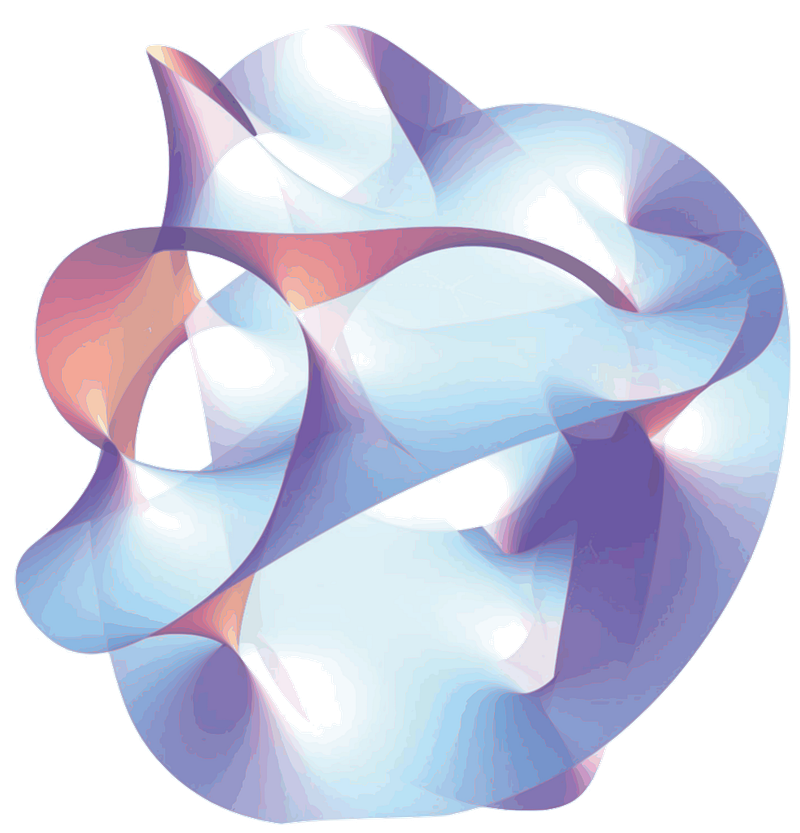
\includegraphics[width=0.35\textwidth]{reduction.png} \quad \quad}
        \vspace{2.5 cm}


        \leftline{ \small { \textbf{Internship tutor:} M. Henning Samtleben}}
        \leftline{ \small { \textbf{Referent teacher:} M. Stéphane Douin}}
        \vspace{1 cm}
        \leftline{\small { \textbf{Educational institution:} Université Paris-Saclay / Magistère de physique fondamentale d'Orsay}}
        \leftline{\small { \textbf{Internship host institution:} Laboratoire de Physique (UMR CNRS 5672), ENS de Lyon}}
        
        \noindent\rule[0.25\baselineskip]{\textwidth}{1pt}\\
        
        {
\includegraphics[width=0.25\textwidth]{logo.png}\quad}
        {
\includegraphics[width=0.2\textwidth]{Logo_Université_Paris-Saclay_(externe).png}\quad}\\
      
    \end{center}
\end{titlepage}
\restoregeometry


\section*{Acknowledgment}
I would like to express my deepest gratitude to Camille Eloy for accepting me into this internship and providing exceptional mentorship. 
Every question I had was met with patience and insight, and through his guidance, 
I had the opportunity to explore the fascinating world of theoretical physics research. I am especially grateful for the chance to delve deeper into theoretical gravity, a field I aspire to work in.
I also extend my sincere thanks to Henning Samtleben for agreeing to supervise this internship.
What made this experience particularly rewarding was the welcoming and supportive environment of the Theory and Models group. Their kindness and readiness to assist made the internship not only enjoyable but also deeply enriching.
For these reasons, I am truly thankful to the entire Theory and Models group for their warm welcome and unwavering support.
\section*{Notations and Abbreviations}
For quick reference, we summarize here the index conventions used throughout this report, following \cite{scherk1979get}; their motivation is explained in Section~\ref{spinconnexionvielbeinandflatspace}.
\begin{itemize} \label{notation}
    \item Hatted Greek letters denote curved indices $(\hat \mu , \hat \nu , \hat \rho , \dots)$.
    \item Hatted Latin letters denote flat indices $(\hat p , \hat m , \hat n , \dots)$.
    \item For space-time indices taking $D$ values, late Greek letters are used in the curved case $(\mu, \nu ,\rho , \dots)$ and Latin letters in the flat case $(p, m, n)$.
    \item For internal indices taking $E$ values, early Greek letters are used in the curved case $(\alpha, \beta ,\gamma , \dots)$ and Latin letters in the flat case $(a,b,c)$.
\end{itemize}
\addcontentsline{toc}{section}{Notation and abbreviations}
\section*{Résumé}

Ce stage a été effectué dans le groupe Théorie et Modèles du Laboratoire de Physique (UMR CNRS 5672) de l'ENS de Lyon, sous la direction du Dr Camille Eloy. 
Il porte sur la réduction dimensionnelle en supergravité et sur l'apparition de symétries de dualité cachées. 
On commence par poser le cadre de la théorie des champs lagrangienne et par introduire le formalisme du vielbein, qui est nécessaire pour bien traiter les indices plats et courbes. 
On reprend ensuite la méthode de Scherk et Schwarz pour réduire l'action NS-NS de la supergravité, écrite en dimension $D+E$, jusqu'en dimension $D$, 
en supposant qu'aucun champ ne dépend des coordonnées internes. La réduction du terme d'Einstein--Hilbert fait apparaître, en plus de la gravité usuelle en dimension $D$, 
$E$ champs de jauge et une matrice de champs scalaires $h_{\alpha\beta}$ qui décrit la géométrie de l'espace interne. La réduction du dilaton mène à un dilaton décalé invariant, 
et celle de la deux-forme fait apparaître un second champ de jauge ainsi qu'une deux-forme réduite. En regroupant $h_{\alpha\beta}$ et la deux-forme réduite dans une seule matrice $M$, 
on montre que l'action complète est invariante sous un groupe $O(E,E)$ qui agit sur $M$ et sur les champs de jauge, une symétrie qu'on ne voit pas du tout dans la théorie non réduite.

\section*{Summary}

This internship was carried out in the Theory and Models group of the Laboratoire de Physique (UMR CNRS 5672) at ENS de Lyon, under the supervision of Dr Camille Eloy. It looks at dimensional reduction in supergravity and at the appearance of hidden duality symmetries. 
We start by laying out Lagrangian field theory and introducing the vielbein formalism, which is needed to properly handle flat and curved indices. 
We then follow the method of Scherk and Schwarz to reduce the NS-NS action of supergravity, written in $D+E$ dimensions, down to $D$ dimensions, assuming that no field depends on the internal coordinates. 
Reducing the Einstein--Hilbert term gives, in addition to ordinary $D$-dimensional gravity, $E$ gauge fields and a scalar matrix $h_{\alpha\beta}$ that describes the geometry of the internal space. 
Reducing the dilaton leads to an invariant shifted dilaton, and reducing the two-form gives a second gauge field along with a reduced two-form. By putting $h_{\alpha\beta}$ and the reduced two-form together into a single matrix $M$, we show that the complete action is invariant under an $O(E,E)$ group acting on $M$ and on the gauge fields, a symmetry that is completely hidden in the unreduced theory.
\newpage

\tableofcontents
\clearpage
\pagenumbering{arabic} 
\section{Introduction}
\subsection{Context of the internship}
This internship was carried out in the Theory and Models group of the physics laboratory of ENS Lyon. It was officially done under the supervision of Henning Samtleben, 
however unofficially the internship was done under the supervision of Camille Eloy, 
who has a postdoctoral position here. He was the one who chose the subject and the person who answered most of the questions I had during this internship.
\subsection{Introduction to the subject}
Since the 19th-century unification of electricity and magnetism,
and the later development of classical and quantum field theory,
physicists have been looking for a single mathematical framework that could describe all fundamental interactions at once.
A great deal of progress has been made for the electromagnetic,
weak, and strong forces, which are now successfully unified in the Standard Model. Gravity, however,
remains the main stumbling block: indeed, its description by General Relativity \cite{einstein1915allgemeinen}
sits completely apart from the quantum field-theoretic language we use for every other force.
One way to address this issue is to add a new symmetry to nature, supersymmetry, which postulates a symmetry mixing the degrees of freedom of fermions and bosons. This symmetry is mainly used in two theories: the first is supergravity, which, as the name
suggests, attempts to combine the principle of supersymmetry with General Relativity. The other major theory is string theory, which, contrary to particle physics, which focuses on point particles, describes the motion of one-dimensional objects called strings.
Both theories describe the existence of extra dimensions. We will focus here on the case of supergravity.\\
The tool we use to make the role of these extra dimensions manifest is dimensional reduction, in the spirit of the original Kaluza--Klein idea: a theory living in $D+E$ dimensions can be reinterpreted, by a $D$-dimensional observer, as a theory in $D$ dimensions containing extra scalar and vector fields that encode the geometry of the $E$ hidden dimensions. Carrying this out consistently and identifying what those extra fields are is the main technical goal of this internship, and it is what ultimately allows us to uncover a hidden symmetry relating theories that look different in $D+E$ dimensions but turn out to be equivalent once reduced.\\
Concretely, we begin by describing what a field theory is, in order to work out how to write down the actions of the fields we will use. We then follow the steps of \cite{scherk1979get} by performing a dimensional reduction from $D+E$ dimensions down to $D$ dimensions. However, following \cite{maharana1993noncompact}, we do not simply use the classical Einstein action,
but the NS-NS action of supergravity, which adds two new fields. We do this using the vielbein formalism, as it is useful for the description of fermions, even though here we only describe bosonic fields.
We then show that, although in high dimensions only the $SL(E,\mathbb{R})$ symmetry is detectable without much work, an additional $O(E,E)$ symmetry appears once we go to low dimensions; this means that
a number of theories that look distinct in $D+E$ dimensions are in fact equivalent.\\
\section{Lagrangian Field Theory}
\subsection{Lagrangian Density}
In this internship we are going to use Lagrangian field theory to describe the objects we will be working with. The main interest of this framework is that it lets us work with an infinite number of degrees of freedom.
To better understand what we are going to do, we are going to follow the same path as \cite{goldstein1950classical}, going from a simple case and then generalizing. Let us start from a simple case in 1D, which we will then generalize to $N$ dimensions. The "simple" example is going to be an infinitely long elastic rod undergoing small
longitudinal vibrations. We can model this with a system of discrete points of equal mass, connected by springs of natural length $a$, as shown in Figure~\ref{fig:latticechain}. Point $i$ is displaced from its equilibrium position by a quantity $\eta_i$.
\begin{figure}[H]
    \centering
    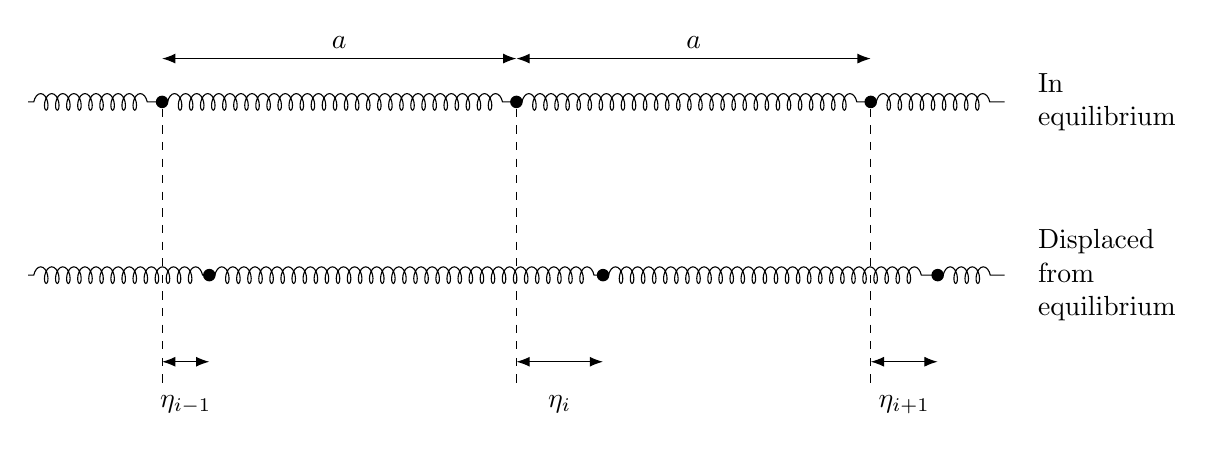
\begin{tikzpicture}[
      spring/.style={decorate, decoration={coil, aspect=0.5, segment length=4pt, amplitude=3pt, pre length=2pt, post length=2pt}},
      dot/.style={circle, fill=black, inner sep=1.6pt},
      >=Latex
    ]

    % ---- vertical positions ----
    \def\ytop{2.2}
    \def\ybot{0}

    % ---- equilibrium mass positions ----
    \def\xa{0}
    \def\xb{4.5}
    \def\xc{9}

    % ================= TOP ROW: in equilibrium =================
    \draw[spring] (-1.7,\ytop) -- (\xa,\ytop);
    \draw[spring] (\xa,\ytop) -- (\xb,\ytop);
    \draw[spring] (\xb,\ytop) -- (\xc,\ytop);
    \draw[spring] (\xc,\ytop) -- (10.7,\ytop);

    \node[dot] (A) at (\xa,\ytop) {};
    \node[dot] (B) at (\xb,\ytop) {};
    \node[dot] (C) at (\xc,\ytop) {};

    % spacing labels "a"
    \draw[<->] (\xa,{\ytop+0.55}) -- (\xb,{\ytop+0.55}) node[midway,above,font=\itshape] {$a$};
    \draw[<->] (\xb,{\ytop+0.55}) -- (\xc,{\ytop+0.55}) node[midway,above,font=\itshape] {$a$};

    \node[anchor=west, align=left] at (11,\ytop) {In\\ equilibrium};

    % ================= BOTTOM ROW: displaced =================
    \def\da{0.6}
    \def\db{1.1}
    \def\dc{0.85}

    \draw[spring] (-1.7,\ybot) -- ({\xa+\da},\ybot);
    \draw[spring] ({\xa+\da},\ybot) -- ({\xb+\db},\ybot);
    \draw[spring] ({\xb+\db},\ybot) -- ({\xc+\dc},\ybot);
    \draw[spring] ({\xc+\dc},\ybot) -- (10.7,\ybot);

    \node[dot] (A2) at ({\xa+\da},\ybot) {};
    \node[dot] (B2) at ({\xb+\db},\ybot) {};
    \node[dot] (C2) at ({\xc+\dc},\ybot) {};

    \node[anchor=west, align=left] at (11,\ybot) {Displaced\\ from\\ equilibrium};

    % ================= dashed reference lines + eta arrows =================
    \draw[dashed] (A) -- (\xa,-1.4);
    \draw[dashed] (B) -- (\xb,-1.4);
    \draw[dashed] (C) -- (\xc,-1.4);

    \draw[<->] (\xa,-1.1) -- ({\xa+\da},-1.1);
    \node[below] at ({(\xa+\xa+\da)/2},-1.4) {$\eta_{i-1}$};

    \draw[<->] (\xb,-1.1) -- ({\xb+\db},-1.1);
    \node[below] at ({(\xb+\xb+\db)/2},-1.4) {$\eta_{i}$};

    \draw[<->] (\xc,-1.1) -- ({\xc+\dc},-1.1);
    \node[below] at ({(\xc+\xc+\dc)/2},-1.4) {$\eta_{i+1}$};

    \end{tikzpicture}
    \caption{A discrete chain of equal masses connected by springs of natural length $a$. Top: the chain at equilibrium. Bottom: the chain displaced from equilibrium, with $\eta_i$ the displacement of mass $i$. (This figure has been produced with the help of Claude AI)}
    \label{fig:latticechain}
\end{figure}
We can then obtain the potential and kinetic energy as
\begin{subequations}
    \begin{align}
        V &= \frac{1}{2}\sum_i m\dot{\eta}_i^2,\\
        T & = \frac{1}{2}\sum_i k(\eta_{i+1} - \eta_i)^2,
    \end{align}
\end{subequations}
and now we can write the Lagrangian of the system, which is
\begin{equation*}
    L = T - V = \frac{1}{2} \sum_i  \Big[ m \dot{\eta}_i^2 - k(\eta_{i+1} - \eta_i)^2\Big],
\end{equation*}
which can be rewritten as
\begin{equation}
    L = T - V = \frac{1}{2} \sum_i a\Big[ \frac{m}{a}\dot{\eta}_i^2 - ak\Big(\frac{\eta_{i+1} - \eta_i}{a}\Big)^2 \Big] = \sum_i a\underbrace{L_i}_{\mathclap{\text{Lagrangian per unit of length of a point.}}}.
\end{equation}
From this we obtain
\begin{equation*}
    \frac{m}{a} \ddot{\eta}_i^2 -ka \Big(\frac{\eta_{i+1} - \eta_i}{a}\Big)^2 + ka \Big(\frac{\eta_{i} - \eta_{i-1}}{a}\Big)^2 =0
\end{equation*}
as the equation of motion for each $\eta_i$.
If we pass to the limit $a\rightarrow 0$, we can see that $\frac{m}{a}\rightarrow \mu$, which is the mass per unit length.
The limit of $ka$ is far less evident, and to determine it we have to use Hooke's law, since we have an elastic rod,
for which the extension of the rod per unit length is proportional to the applied force. Thus the relation is
\begin{equation}
    F= Y \xi,
\end{equation}
where $\xi$ is the elongation per unit length and $Y$ is Young's modulus. Now we can write $\xi = \frac{\eta_{i+1} - \eta_i}{a}$. The force necessary to
stretch the spring by this amount is
\begin{equation*}
    F = k(\eta_{i+1} - \eta_i) = ka \Big(\frac{\eta_{i+1} - \eta_i}{a}\Big) = ka \xi,
\end{equation*}
which means that $ka$ is the Young's modulus of the continuous rod. As we go from the discrete to the continuous case, the integer $i$ identifying 
the particular mass point becomes the continuous position coordinate $x$. We now have $\eta(x)$ instead of $\eta_i$.
Furthermore, as $a$ goes to zero, we have
\begin{equation*}
    \frac{\eta_{i+1} - \eta_i}{a} = \frac{\eta(x+a) - \eta(x)}{a} \underset{a \rightarrow 0}\rightarrow \dv{\eta}{x},
\end{equation*}
since $a$ was playing the role of $dx$. As it approaches zero, the sum we had earlier turns into an integral over the length of the rod, and the Lagrangian
becomes
\begin{equation}
    L = \frac{1}{2} \int \Big[ \mu \dot{\eta}^2 - Y\Big(\dv{\eta}{x}\Big)^2 \Big] dx.
\end{equation}
In the limit $a \rightarrow 0$ the last two terms of the equation of motion become
\begin{equation*}
    \lim_{a \rightarrow 0} - \frac{Y}{a} \Big[ \left.\dv{\eta}{x} \right|_x - \left.\dv{\eta}{x}\right|_{x-a} \Big],
\end{equation*}
which is, in effect, a second derivative of $\eta$. Hence, the equation of motion for the continuous case is
\begin{equation}
    \mu \dv[2]{\eta}{t} - Y \dv[2]{\eta}{x} = 0,
\end{equation}
which is the wave equation in one dimension, with propagation velocity
\begin{equation*}
    v = \sqrt{\frac{Y}{\mu}}.
\end{equation*}
And so we recover d'Alembert's equation.
Now we can see that, even though we have an infinite number of points, there is not an infinite number of Lagrange equations, but merely one.
This also means that we can write the Lagrangian as
\begin{equation*}
    L = \int\mathcal{L} \, dx,
\end{equation*}
where here $\mathcal{L}$ is the Lagrangian per unit length. This generalizes to $ND$, where
the Lagrangian can be written as
\begin{equation} \label{densitylagrandef}
    L = \iiint \mathcal{L}(\eta_{\rho},\pdv{\eta_{\rho}}{x^{\nu}}) \, dx^N.
\end{equation}
Now, if we want to use General Relativity we have to modify the measure by adding a $\sqrt{g}$, so the action, for example, will be,
\begin{equation} \label{actiondensitylag}
    S = \int \sqrt{g} \mathcal{L} \, dx^{N}dt.
\end{equation}
As a final note, one can see that both the variational method and the Lagrangian formalism work in the same way as before the transformation. \footnote{We establish the Lagrangian equation in appendix \ref{Euler-Lag}}
\subsection{General example for scalar and vector fields, and Two-Forms fields}
In field theory, the Lagrangian has a classical form for any field (often the simplest case).
For this work, only the scalar, vector, and two-form Lagrangians are needed, along with the metric, which is handled by Einstein's equations. Furthermore, we will only consider free fields.
So, for a scalar field we have
\begin{equation} \label{scalafield}
    \boxed{\mathcal{L} = - \frac{1}{2} \partial_\mu \Phi \partial^ \mu \Phi,}
\end{equation}
which gives us $\square \Phi =0$ as the equation of motion.
And for a vector field we have
\begin{equation}\label{vectorialfield}
    \boxed{\mathcal{L} = - \frac{1}{4}F_{\mu \nu}F^{\mu \nu},}
\end{equation}
where, for the field $A$,
\begin{equation*}
    F_{\mu \nu} = \partial_\mu A_\nu - \partial_\nu A_\mu.
\end{equation*}
The equation of motion is $\partial_\mu F^{\mu \nu} = 0$, which is exactly two Maxwell's equations, namely Gauss and Ampère. Another thing to remark is that, as $F_{\mu \nu}$ is antisymmetric with its index, that means that the Lagrangian is symmetric with its index.
In vacuum, the Einstein equation gives us
\begin{equation*} \label{einsteinaction}
    \boxed{\mathcal{L} = R,}
\end{equation*}
where $R$ is the Ricci scalar, and the equation of motion is exactly Einstein's equation.
Finally, for the Lagrangian of a two-form field
we have
\begin{equation} \label{Baction}
    \boxed{\mathcal{L} = \frac{1}{12} H_{ \mu \nu \rho}H^{ \mu\nu \rho},}
\end{equation}
where, for the two-form $B_{\nu \rho}$, which is antisymmetric, we also have
\begin{equation*}
    H_{ \mu \nu \rho} = \partial_ \mu B_{\nu \rho} + \text{cyclic permutations},
\end{equation*}
which means that $H$ is antisymmetric under the exchange of any two indices, and it has cyclic symmetry.
and the equation of motion is $\partial_\mu H^{\mu \nu\rho} = 0$.
\subsection{NS-NS Action of Supergravity}
With these objects we can construct the NS-NS action, which has the form
\begin{equation} \label{NS-NSaction}
    \boxed{S = \int d x^D \int \frac{d y ^E}{\rho(E)}\sqrt{- \hat g } e^{ - \hat \phi} \Big(\hat R +  \partial_{\hat \mu}\hat \phi \partial^{\hat \mu}\hat \phi - \frac{1}{12}  H_{ \mu \nu \rho}H^{ \mu\nu \rho}\Big),}
\end{equation} 
where $x^D$ represents the space-time coordinates, $y^E$ the internal space coordinates, and $\rho(E)$ is a normalization factor (i.e., the volume of the internal space), corresponding in practice to the invariant volume of the internal space,
and where $\hat R$ is similar to the classical Einstein--Hilbert action but in $D+E$ dimensions, $\hat \phi$ is a scalar field named the dilaton, and $- \frac{1}{12} H_{ \mu \nu \rho}H^{ \mu\nu \rho}$ is the action of a two-form.
We will now separate this action into two main parts.
Now that we have this action in $D+E$ dimensions, we need, as in \cite{scherk1979get}, to reduce it, which basically means looking at how a $D$-dimensional observer
would perceive those extra dimensions. We will work in the simplest setting: we assume that none of the fields depend on the internal coordinates, so that for any field we have $\partial_\alpha A^{\hat \mu} = 0$.
Finally, since no field depends on the internal coordinates, and given $\rho(E)$, we can simplify this integral.
We can separate the action into two main components: one being the gravitational part with the dilaton, and the other being the two-form part. So we have
\begin{subequations}
    \begin{align}
        &S_{\hat g} = \int d x^D\sqrt{- \hat g } e^{-\hat \phi} \big[\hat R +\partial_{\hat \mu}\hat \phi \partial^{\hat \mu}\hat \phi\big], \label{Sg}\\ 
        &S_{\hat B} =  \int d x^D \sqrt{- \hat g } e^{-\hat \phi} \Big(- \frac{1}{12} H_{ \mu \nu \rho}H^{ \mu\nu \rho}\Big). \label{SB}
    \end{align}
\end{subequations}
\clearpage
\section{Gravitational Action Reduction}
We will begin with the gravitational part of the NS-NS action.
\subsection{Vielbein Formalism} \label{spinconnexionvielbeinandflatspace}
In General Relativity \footnote{We are going to present some reminder of general relativity in appendix \ref{RGreminder}.} we often encounter metrics that are difficult to handle, such as the Kerr--Newman metric. A useful idea is then to work in an orthonormal basis $\{V^a_\mu \}$, which satisfies
\begin{equation} \label{vieldef}
    g_{\mu \nu} V^{\mu}_{a}V^{\nu}_b = \eta_{ab},
\end{equation}
where $g$ is the original metric and $\eta$ is the Minkowski metric.
We call this basis the vielbein. In this basis, indices are raised and lowered using the Minkowski metric.
The dual basis, also called the inverse vielbein, is defined by
\begin{equation} \label{inversviel}
    V^{a}_{\nu}V^{\nu}_b = \delta^a_b.
\end{equation}
Consequently, the curved metric can be reconstructed from the vielbein:
\begin{equation} \label{toflatmet}
    g_{\mu \nu} = \eta_{ab}V^{a}_{\mu}V^{b}_\nu.
\end{equation}

The vielbein also allows us to transform vectors, covectors, and tensors between curved and flat indices:
\begin{align} \label{changeofbasis}
    T^a &= V^a_\mu T^\mu, \\
    T_a &= V^\mu_a T_\mu, \\
    T^a_b &= V^a_\mu V^\nu_b T^\mu_\nu.
\end{align}
The introduction of flat indices requires a corresponding modification of the usual transformation law. In particular, the Christoffel connection must be replaced by the spin connection, defined by
\begin{equation} \label{spinconnexion}
    \nabla_\mu X^a_b =
    \partial_\mu X^a_b
    + \omega_\mu{}^a{}_c X^c_b
    - \omega_\mu{}^c{}_b X^a_c.
\end{equation}
The spin connection remains related to the Levi--Civita connection through
\begin{align} \label{linkbetwinleviandlatin}
    \Gamma_{\mu \lambda}^{\nu}
    &= V^{\nu}_a \partial_\mu V^a_\lambda
    + V^\nu_aV^b_\lambda \omega_\mu{}^a{}_b,\\
    \omega_\mu{}^a{}_b
    &= V^a_\nu V^\lambda_b \Gamma_{\mu \lambda}^{\nu}
    - V^\lambda_b \partial_\mu V^a_\lambda.
\end{align}
With these relations we can prove the antisymmetry of the last two indices of the spin connection:
\begin{equation}
    \begin{aligned}
        \nabla_\mu \eta_{ab} &= \partial_\mu X_{ab} - \omega_\mu{}^a{}_c \eta_{cb} - \omega_\mu{}^c{}_b \eta_{ac} \\
        &=  - \omega_{\mu a b } - \omega_{\mu b a}\\
        & = 0.
    \end{aligned}
\end{equation}
So, in effect, we have
\begin{equation} \label{antisymlat}
    - \omega_{\mu a b }= \omega_{\mu b a}.
\end{equation}
Throughout this reduction we will use the vielbein formalism, following the same notation as in \cite{scherk1979get} (summarized on page~\pageref{notation}): 
hatted Greek letters $(\hat \mu , \hat \nu , \hat \rho , \dots)$ denote curved indices and hatted Latin letters $(\hat p , \hat m , \hat n , \dots)$ denote flat indices; among these, 
the $D$ space-time directions are labelled by late Greek letters $(\mu, \nu, \rho, \dots)$ in the curved case and late Latin letters $(p, m, n)$ in the flat case, 
while the $E$ internal directions are labelled by early Greek letters $(\alpha, \beta, \gamma, \dots)$ in the curved case and early Latin letters $(a, b, c)$ in the flat case. 
The general coordinate $x^{\hat \mu}$ is therefore made up of a space-time coordinate $x^\mu$ and an internal coordinate $y^\alpha$. 
The flat Lorentz indices are precisely the ones on which the vielbein formalism, 
introduced below, lets us use the flat Minkowski metric $\eta_{ab}$ to raise and lower indices, in place of the curved metric $g_{\mu \nu}$.
\subsection{Rewriting the Action}
For this part we do not need the $\hat g^{\hat \mu \hat \nu}\partial_{\hat \mu}\hat \phi \partial^{\hat \nu}\hat \phi$ part of the action, so we will ignore it entirely.
Now, using the fact that $\hat R$ can be written as
\begin{equation*} \label{Ricciexp}
    \hat R = \hat V^{\hat \mu \hat r} \hat V^{\hat \nu \hat s} \hat R_{\hat \mu \hat \nu \hat r \hat s},
\end{equation*}
where 
\begin{equation*} \label{expriemann}
    \hat R_{\hat \mu \hat \nu \hat r \hat s} =  \partial_{\hat \mu } \hat \omega_{\hat \nu \hat r \hat s}+ \hat \omega_{\hat\mu \hat r}{}^{\hat t}\omega_{\hat\nu \hat t \hat s} - (\mu \leftrightarrow \nu),
\end{equation*}
and the $\omega$'s are defined by
\begin{equation} \label{expomega}
    \hat \omega_{trs } = - \hat\Omega_{\hat t\hat r \hat s} +\hat\Omega_{\hat r\hat s \hat t } -\hat\Omega_{\hat s\hat t \hat r},
\end{equation}
and finally the $\Omega$'s are defined via the vielbein by
\begin{equation}\label{expOmega}
    \hat\Omega_{\hat r\hat s \hat t } = \frac{1}{2}\big(\hat V^{\hat \mu}_{\hat r}\hat V^{\hat \nu}_{\hat s} -\hat V^{\hat \nu}_{\hat r} \hat V^{\hat \mu}_{\hat s}\big)\partial_{\hat \nu} \hat V_{\hat \mu \hat r},
\end{equation}
with all of that we can now rewrite the action $S_{\hat g}$ in terms of $\hat \omega$:
\begin{align}
    S_{\hat g} &= \int d x^D\hat V  e^{-\hat \phi} \hat R \nonumber \\
    &= \int d x^D\hat V  e^{-\hat \phi} \hat V^{\hat \mu \hat r} \hat V^{\hat \nu \hat s} \hat R_{\hat \mu \hat \nu \hat r \hat s} \nonumber \\
    &= \int d x^D\hat V e^{-\hat \phi} \hat V^{\hat \mu \hat r} \hat V^{\hat \nu \hat s} \left([\partial_{\hat \mu } \hat \omega_{\hat \nu \hat r \hat s} -\partial_{\hat \nu } \hat \omega_{\hat \mu \hat r \hat s}]+ [\hat \omega_{\hat\mu \hat r}{}^{\hat t}\omega_{\hat\nu \hat t \hat s} - \hat \omega_{\hat\nu \hat r}{}^{\hat t}\omega_{\hat\mu \hat t \hat s}]\right) \nonumber\\
    &\text{Integrating the first two terms by parts and dropping the resulting boundary term,} \nonumber \\
    &= \int d x^D\{  \hat V e^{-\hat \phi}[\hat \omega^{\hat r}{}_{\hat r}{}^{\hat t}\omega^{\hat s}{}_{\hat t \hat s} - \hat \omega^{\hat s}{}_{ \hat r}{}^{\hat t}\omega^{\hat r}{}_{ \hat t \hat s}]- 2\hat \omega_{\hat \nu \hat r \hat s}[\hat V e^{-\hat \phi} \hat V^{\hat \mu \hat r} \partial_{\hat \mu} \hat V^{\hat \nu \hat s} +\hat V e^{-\hat \phi}
    \hat V^{\hat \nu \hat s} \partial_{\hat \mu}\hat V^{\hat \mu \hat r}+ e^{-\hat \phi} \hat V^{\hat \mu \hat r} \hat V^{\hat \nu \hat s} \partial_{\hat \mu}\hat V +\hat V  \hat V^{\hat \mu \hat r} \hat V^{\hat \nu \hat s} \partial_{\hat \mu}e^{-\hat \phi} ] \} \nonumber \\
    &\text{Using the raising/lowering rules and the equation above to simplify,} \nonumber \\
    &= \int d x^D\hat V e^{-\hat \phi} \{  \hat \omega^{\hat s}{}_{\hat s}{}^{\hat t}\omega^{\hat r}{}_{\hat r \hat t} + \hat \omega^{\hat s \hat t}{}_{ \hat r}\omega^{\hat r}{}_{  \hat s \hat t }+ 2\hat \omega_{\hat s}{}^{\hat r \hat s}\hat V^{\hat \mu}_{ \hat r}\partial_{\hat \mu}\hat \phi \}.
\end{align}
\subsection{Vielbein Ansatz} \label{part:vielbeinanstaz}
Now that we have explicitly written the action in terms of the Latin connection and the two other fields, what remains is to assume an ansatz for the vielbein. Why the vielbein and not the metric, one may ask? Because, as stated in Section~\ref{spinconnexionvielbeinandflatspace},
all the information contained in the metric is also contained in the vielbein, and since we primarily work with the vielbein in the action, it is easier to formulate the ansatz on it. We now use the same ansatz as in \cite{scherk1979get},
except that we use the same parameter conventions as in \cite{maharana1993noncompact}. Finally, thanks to local Lorentz invariance we can choose a triangular parametrization, giving us
\begin{equation} \label{vielbeinanstaz}
    \boxed{\hat V^{\hat r}_{\hat \mu} =\begin{pmatrix}
    V^{r}_{\mu} & A^{(1)\beta }_{\mu} \Phi^{a}_{\beta} \\ 0 & \Phi^{a}_\alpha
    \end{pmatrix}. }
\end{equation}
Now, still using \eqref{inversviel}, we can compute the inverse vielbein and then the metric and inverse metric, which gives us
\begin{equation} \label{expinverseviel}
    \hat V^{\hat \mu}_{\hat r} = \begin{pmatrix} 
         V^\mu_r &  - A^{(1)\alpha }_r \\ 0 & \Phi^\alpha_a
    \end{pmatrix}
\end{equation}
for the inverse vielbein, and
\begin{equation} \label{expmetric}
    \hat g_{\hat \mu \hat \nu} = \begin{pmatrix}
        g_{\mu \nu} - A^{\gamma}_{\mu}A^{(1)}_{\nu \lambda} & - A^{(1)}_{\mu \beta} \\  A^{(1)}_{\nu \alpha} &-h_{\alpha \beta}
    \end{pmatrix}, \quad
    \hat g^{\hat \mu \hat \nu} = \begin{pmatrix}
        g^{\mu \nu}  & - A^{ (1)\mu \beta} \\ - A^{(1)\nu \alpha} &-h^{\alpha \beta}+ A^{(1)\beta}_{\rho}A^{\rho \alpha}
    \end{pmatrix}
\end{equation}
for the metric. Here $h_{\alpha \beta}$ is the internal space metric and its vielbein is $\Phi^a_\alpha$. This means that $h_{\alpha \beta} = \Phi^a_\alpha \delta_{a b } \Phi^b_\beta $. We will denote its determinant by $h$.
\subsection{Gauge Observation} \label{part:gaugeviel}
Now that we have set up the ansatz, we would like to identify what each object is. To that end, we can use the classical gauge transformation $x'^\mu = x^\mu + \Lambda^{(1)\mu}(x)$ and use the fact that it can easily be rewritten as a Lie derivative.
Indeed, since we already know how different objects transform under a Lie derivative, we can easily identify what each object is.
So, firstly, let us list every known transformation:
 \begin{align} \label{xitransfo}
    &\delta \phi(x) =L_{\Lambda^{(1)}} \phi(x) = \Lambda^ {(1)\mu} \partial _ \mu \Phi (x), \\
    &\delta U ^ \mu  =L_{\Lambda^{(1)}} U ^ \mu = \Lambda^{(1)\rho} \partial _ \rho U ^ \mu - (\partial _ \rho \Lambda^{(1)\mu}) U ^\rho, \\
    &\delta  \omega _ \mu  =L_{\Lambda^{(1)}} \omega _ \mu  =  \Lambda^{(1)\rho} \partial _ \rho \omega _\mu + (\partial _ \rho \Lambda^{(1)\mu}) \omega _\rho, \\
    &\delta T ^ \mu _ \nu  =L_{\Lambda^{(1)}} T ^ \mu _ \nu =\Lambda^{(1)\rho}  \partial _ \rho T ^ \mu _ \nu -(\partial _ \rho \Lambda^{(1)\mu} ) T ^ \rho _ \nu + (\partial _ \nu \Lambda^{(1)\rho})T ^ \mu _ \nu. 
\end{align} 
We now apply the transformation to each block of the vielbein, in order to see whether it corresponds to some familiar type of field, still using \eqref{xitransfo}. Let us start with the block $\hat V^r_\mu$:
\begin{align*}
    \delta \hat V^r_\mu &= \delta V^r_\mu=  \Lambda^{(1)\hat \rho}  \partial_{\hat \rho} \hat V^{ r}_{ \mu} + \partial_{ \mu} \Lambda^{(1) \hat \rho} \hat V^{  r}_{\hat \rho} \\
   &=  \Lambda^{(1)\hat \rho}  \partial_{\hat \rho} \hat V^{ r}_{ \mu} + \partial_{ \mu} \Lambda^{(1) \hat \nu} \hat V^{  r}_{\hat \nu}\\
   &=  \Lambda^{(1) \rho}  \partial_{ \rho}  V^{ r}_{ \mu} + \partial_{ \mu} \Lambda^{(1)  \nu}  V^{  r}_{ \nu},\\
\end{align*}
which is exactly the transformation law of a vector field under a Lie derivative \cite{freedman2012supergravity}. Applying the same method to the other blocks, we obtain, for $\Phi^a_\alpha$,
\begin{equation*}
    \delta \Phi^a_\alpha = \Lambda^{(1)\rho} \partial_\rho \Phi^a_\alpha,
\end{equation*}
which is exactly the transformation law of a scalar field. Finally, for $A^{(1)\alpha}_\mu$ we obtain
\begin{equation*}
    \delta A^{(1)\alpha}_\mu= \Lambda^{(1)\rho}\partial_\rho A^{(1)\alpha}_\mu + \partial_\mu \Lambda^{(1)\rho} A^{(1)\alpha}_\rho +\partial_\mu \Lambda^{(1)\alpha},
\end{equation*}
which corresponds to the transformation law of a vector field, up to an extra correction term. One may further note that, restricting to $\xi^\alpha$ only, we obtain
\begin{subequations}
\begin{align}
&\delta V^r_\mu = \delta \Phi^a_\alpha = 0,\\
&\delta A^{(1)\alpha}_\mu = \partial_\mu \Lambda^{(1)\alpha} .
\end{align}
\end{subequations}
So, what remains of the $D$-dimensional diffeomorphisms, once restricted to $\xi^\alpha$ independent of the internal coordinates $y$, corresponds to a set of $E$ abelian gauge symmetries.
The vielbein in \eqref{vielbeinanstaz} thus contains the $D$-dimensional vielbein (i.e., the graviton), $E$ vector fields $A^{(1)\alpha}_\mu$, and $E^2$ scalar fields $\Phi^a_\alpha$. However, because of local Lorentz invariance in the internal directions, only $\frac{1}{2}E(E+1)$ of these scalars actually correspond to propagating degrees of freedom. We also introduce $\delta = \det \Phi$. 
\subsection{Ricci Scalar Reduction}
Now that we are better acquainted with the tools we will use, we can begin the calculation. To start, we consider the Einstein action in $D+E$ dimensions, modified by the addition of the dilaton.\\
First, let us fully expand $S_{\hat g}$: this shows that we technically need to compute 8 $\omega$'s; however, thanks to the antisymmetry of the last two indices, this reduces to 6.
So the action is
\begin{equation} \label{Sdexp}
\boxed{
  \begin{aligned}
S=&\int d^{D}x\,\hat V\,e^{-\phi} \,\Big[\;
\hat\omega^a{}_{b  c}\hat \omega^{bc}{}_a
-\hat \omega^a{}_{t  b}\hat \omega^{bt}{}_a
+\hat\omega^a{}_{s  c}\hat\omega^{sc}{}_a
+\hat\omega^a{}_{s  t}\hat\omega^{st}{}_a
-\hat\omega^r{}_{b  c}\hat\omega^{b}{}_r{}^c
-\hat\omega^r{}_{t  b}\hat\omega^{bt}{}_r
-\hat\omega^r{}_{s  c}\hat\omega^{s}{}_r{}^c \\
&-\hat\omega^r{}_{s  t}\hat\omega^{st}{}_r
+\hat\omega^a{}_{ac}\hat\omega^b{}_b{}^c
+\hat\omega^a{}_{ta}\hat\omega^b{}^t{}_b
+\hat\omega^a{}_{ac}\hat\omega^s{}_s{}^c 
-\hat\omega^a{}_{ta}\hat\omega^s{}_s{}^t
+\hat\omega^r{}_{rc}\hat\omega^b{}_b{}^c
-\hat\omega^r{}_{rt}\hat\omega^b{}^t{}_b
+\hat\omega^r{}_{rc}\hat\omega^s{}_s{}^c
+\hat\omega^r{}_{rt}\hat\omega^s{}_s{}^t\\
&+2\hat \omega_{ s}{}^{ r  s}\hat V^{ \mu}_{  r}\partial_{ \mu}\hat \phi
+2\hat \omega_{ b}{}^{ r  b}\hat V^{ \mu}_{  r}\partial_{ \mu}\hat \phi
\;\Big]
\end{aligned}}
\end{equation}
It then becomes clear that we only need to compute six components of $\omega$, namely
\begin{align*}
    &\hat \omega_{pmn}, \;
    \hat \omega_{pma}, \;
    \hat \omega_{pab},\\
    &\hat \omega_{cmn},\;
    \hat \omega_{cma},\;
    \hat \omega_{cab}.\;
\end{align*}
One can also check that computing these six components only requires the following eight components of $\Omega$:
\begin{align*}
    &\hat \Omega_{pmn},\\
    &\hat \Omega_{pma},\;
    \hat \Omega_{pam},\;
    \hat \Omega_{apm},\\
    &\hat \Omega_{mab},\;
    \hat \Omega_{amb},\;
    \hat \Omega_{abm},\\
    &\hat \Omega_{abc}.
\end{align*}
Using \eqref{expinverseviel}, \eqref{expomega} and \eqref{expOmega}, we can now set out a clear strategy: first the $\Omega$'s, then the $\omega$'s.
Let us begin the computation of the $\Omega$'s, starting with $\hat \Omega_{pmn}$:
\begin{align*}
    \hat \Omega_{pmn} &= \frac{1}{2}(\hat V^{\hat \mu}_{  p} \hat V^{ \nu}_{m}-\hat V^{\hat \mu}_{m} \hat V^{ \nu}_{p})\partial_{ \nu} \hat V_{\hat \mu n}\\
    &= \frac{1}{2}(V^{ \mu}_{  p} V^{ \nu}_{m}- V^{ \mu}_{m} V^{ \nu}_{p})\partial_{ \nu} ( V_{ \mu n})\\
    &= \Omega_{pmn}.
\end{align*}
For $\hat \Omega_{pma}$, we find:
\begin{align*}
    \hat \Omega_{pma} &= \frac{1}{2}(\hat V^{\hat \mu}_{  p} \hat V^{ \nu}_{m}-\hat V^{\hat \mu}_{m} \hat V^{ \nu}_{p})\partial_{ \nu} \hat V_{\hat \mu a}\\
    &= -( V^{\mu}_{  p}  V^{ \nu}_{m}-  V^{ \mu}_{m} V^{ \nu}_{p})\partial_{ \nu} (A^{(1)\alpha}_{\mu}\Phi_{a\alpha}) + ( A^{(1)\alpha}_p V^{ \nu}_{m}- A^{(1)\alpha}_{m} V^{ \nu}_{p})\partial_{ \nu} (\Phi_{a\alpha})\\
    &= - (V^{ \mu}_{  p}  V^{ \nu}_{m}- V^{ \mu}_{m}  V^{ \nu}_{p})(\partial_{ \nu} (A^{(1)\alpha}_{\mu})\Phi_{a\alpha}+\partial_{ \nu}(\Phi_{a\alpha})A^{(1)\alpha}_{\mu}) + ( A^{(1)\alpha}_p V^{ \nu}_{m}- A^{(1)\alpha}_{m} V^{ \nu}_{p})\partial_{ \nu} (\Phi_{a\alpha}) \\
    &= - (V^{ \mu}_{  p}  V^{ \nu}_{m}- V^{ \mu}_{m}  V^{ \nu}_{p})\partial_{ \nu} (A^{(1)\alpha}_{\mu})\Phi_{a\alpha}\\
    &=  F^\alpha{}_{pm}\Phi_{a\alpha}- \partial_\nu(V^{ \mu}_{  p}  V^{ \nu}_{m})A^{(1)\alpha}_{\mu}\Phi_{a\alpha}+ \partial_\nu(V^{ \nu}_{  p}  V^{ \mu}_{m})A^{(1)\alpha}_{\mu}\Phi_{a\alpha}\\
    &=  F^\alpha{}_{pm}\Phi_{a\alpha}.
\end{align*}
For $\hat \Omega_{pam}$:
\begin{align*}
    \hat \Omega_{pam} &= \frac{1}{2}(\hat V^{\hat \mu}_{  p} \hat V^{ \nu}_{a}-\hat V^{\hat \mu}_{a} \hat V^{ \nu}_{p})\partial_{ \nu} \hat V_{\hat \mu m}\\
    &= 0.
\end{align*}
The same result holds for $\hat \Omega_{apm}$.\\
For $\hat \Omega_{pab}$:
\begin{align*}
    \hat \Omega_{pab} &= \frac{1}{2}(\hat V^{\hat \mu}_{  p} \hat V^{ \nu}_{a}-\hat V^{\hat \mu}_{a} \hat V^{ \nu}_{p})\partial_{ \nu} \hat V_{\hat \mu b}\\
    &= \frac{-1}{2}\hat V^{\hat \mu}_{a}  V^{ \nu}_{p}\partial_{ \nu} \hat V_{\hat \mu b}\\
    &= \frac{1}{2} \Phi^{ \alpha}_{a}  V^{ \nu}_{p}\partial_{ \nu}  \Phi_{\alpha b}\\
    &= \frac{1}{2} \Phi^{ \alpha}_{a}  V^{ \nu}_{p}\partial_{ \nu}( h_{\alpha \beta} \Phi^{\beta}_{ b})\\
    &= \frac{1}{2} \Phi^{ \alpha}_{a}  \Phi^{\beta}_{ b}V^{ \nu}_{p}\partial_{ \nu} h_{\alpha \beta}  +\frac{1}{2} \Phi^{ \alpha}_{a}  V^{ \nu}_{p}h_{\alpha \beta}\partial_{ \nu}  \Phi^{\beta}_{ b}\\
    &= \frac{1}{2} \Phi^{ \alpha}_{a}  \Phi^{\beta}_{ b}V^{ \nu}_{p}\partial_{ \nu} h_{\alpha \beta}  +\frac{1}{2} \Phi_{\beta a}  V^{ \nu}_{p}\partial_{ \nu}  \Phi^{\beta}_{ b}\\
    &= \frac{1}{2} \Phi^{ \alpha}_{a}  \Phi^{\beta}_{ b}V^{ \nu}_{p}\partial_{ \nu} h_{\alpha \beta}  +\frac{1}{2}   V^{ \nu}_{p}\partial_{ \nu} \big(\underbrace{\Phi_{\beta a} \Phi^{\beta}_{ b}}_{\mathclap{=\delta_{ab},\ \text{i.e. constant}}}\big) - \Phi^{\beta}_{ b} V^{ \nu}_{p}\partial_{ \nu} \Phi_{\beta a} \\
    &=\frac{1}{2} \Phi^{ \alpha}_{a}  \Phi^{\beta}_{ b}V^{ \nu}_{p}\partial_{ \nu} h_{\alpha \beta} - \Phi^{\beta}_{ b} V^{ \nu}_{p}\partial_{ \nu} \Phi_{\beta a}. 
\end{align*}
For $\hat \Omega_{apb}$:
\begin{align*}
    \hat \Omega_{apb} &= \frac{1}{2}(\hat V^{\hat \mu}_{  a} \hat V^{ \nu}_{p}-\hat V^{\hat \mu}_{p} \hat V^{ \nu}_{a})\partial_{ \nu} \hat V_{\hat \mu b}\\
    &= \frac{1}{2}\hat V^{\hat \mu}_{  a} \hat V^{ \nu}_{p}\partial_{ \nu} \hat V_{\hat \mu b}\\
    &= \frac{1}{2}\hat V^{\alpha}_{  a} \hat V^{ \nu}_{p}\partial_{ \nu} \hat V_{\alpha b}\\
    &= \frac{-1}{2} \Phi^{\alpha}_{  a}  V^{ \nu}_{p}\partial_{ \nu} \Phi_{\alpha b}.\\
\end{align*}
For $\hat \Omega_{abp}$:
\begin{align*}
    \hat \Omega_{abp} &= \frac{1}{2}(\hat V^{\hat \mu}_{  a} \hat V^{ \nu}_{b}-\hat V^{\hat \mu}_{b} \hat V^{ \nu}_{a})\partial_{ \nu} \hat V_{\hat \mu p}\\
    &= 0.
\end{align*}
The same holds for $\Omega_{abc}$. Using \eqref{vielbeinanstaz}, we can then obtain the $\omega$'s:

\begin{subequations}
\begin{align}
&\hat\omega_{pmn} = \omega_{pmn},\\
&\hat \omega_{pma} = F^{\alpha}_{pm}\Phi_{\alpha a},\\
&\hat\omega_{pab} = \frac{1}{2}\Phi^\alpha_aV^\mu_p\partial_\mu\Phi_{\alpha \beta} - (a \leftrightarrow b),\\
&\hat\omega_{cmn} = - F^{\alpha}_{mn}\Phi_{\alpha c},\\
&\hat\omega_{cma} = \frac{1}{2}\Phi^\alpha_a \Phi^\beta_cV^\lambda_m\partial_\lambda h_{\alpha \beta},\\
&\hat \omega_{cab}  = 0.
\end{align}
\end{subequations}
We can now conclude this section by carrying out the multiplication from equation \eqref{Sdexp} and examining the result, which gives
\begin{equation}
    \boxed{
    \begin{aligned}
    S_{\hat g} = &\int d x^D e^{-\hat \phi} V \delta \Big( 
    \frac{-1}{4} g^{\rho \lambda} \partial_\lambda h_{\alpha \beta}\partial_\rho h^{\alpha \beta}
    +\frac{1}{4}F^{\mu \nu \alpha}F^{\beta}_{\mu  \nu}h_{\alpha \beta}+\\
    &+ R + \frac{1}{4} \partial_{\hat \mu} \log(h) \partial^{\hat \mu} \log(h) + \partial_{\hat \mu} \log(h) \partial^{\hat \mu} \hat \phi \Big).
\end{aligned}}
\end{equation}
We can observe some interesting things. First, we recover the classical Einstein action, coupled to $E$ electromagnetic fields. So we can conclude that gravity in $D + E $ dimensions, once reduced down to $D$ dimensions, is equivalent to gravity in $D$ dimensions coupled to $E$ electromagnetic fields and scalars.
\subsection{Adding the Dilaton Field Reduction}
For this part we sum $S_{\hat g}$ and $S_{\hat \phi}$, which gives
    \begin{equation*}
    \begin{aligned}
    S_{\hat g + \hat \phi} = &\int d x^D e^{-\hat \phi}V \delta \Big( 
    \frac{-1}{4} g^{\rho \lambda} \partial_\lambda h_{\alpha \beta}\partial_\rho h^{\alpha \beta}
    +\frac{1}{4}F^{\mu \nu \alpha}F^{\beta}_{\mu  \nu}h_{\alpha \beta}+\\
    &+ R + \frac{1}{4} \partial_{\hat \mu} \log(h) \partial^{\hat \mu} \log(h) + \partial_{\hat \mu} \log(h) \partial^{\hat \mu} \hat \phi + \partial_{\hat \mu} \hat \phi \partial^{\hat \mu} \hat \phi \Big).
\end{aligned}
\end{equation*}
We then introduce the shifted dilaton
\begin{equation}
    \phi = \hat \phi -\frac{1}{2} \log{h}= \hat \phi - \log{\delta},
\end{equation}
which gives
\begin{equation}
\boxed{
    \begin{aligned}
    S = &\int d x^D V e^{- \phi}\Big(
    R -\frac{1}{4}F^{\mu \nu \alpha}F^{\beta}_{\mu  \nu}h_{\alpha \beta}+\\
    &- g^{\rho \lambda} \partial_\lambda h_{\alpha \beta}\partial_\rho h^{\alpha \beta}
    + \partial_{ \mu}\phi\partial^{ \mu}\phi\Big).
\end{aligned}}
\end{equation} 
\section{Two-Form Field Reduction}
\subsection{The Reduction}
For the two-form we will carry out the reduction separately from the other two fields; this causes no issue, as the action is linear in it.
We can rewrite \eqref{Baction} as
\begin{align*}
    \mathcal{L}_{\hat B} &= \frac{-1}{12} \hat H_{ \hat \mu \hat \nu \hat \rho} \hat H^{ \hat \mu \hat \nu \hat \rho}\\
    \intertext{Here we use \eqref{changeofbasis} to pass the lower-index $H$ to the flat-space basis, and reuse the identity to change the upper index as well:}
    &=\frac{-1}{12} \hat H_{ \hat r \hat s \hat t}  \hat V^{\hat r}_{\hat \mu} \hat V^{\hat s}_{\hat \nu} \hat V^{\hat t}_{\hat \rho} \hat H^{ \hat \mu \hat \nu \hat \rho}\\
    &=\frac{-1}{12}(\hat H_{ \hat r \hat s\hat t}\hat H^{ \hat r \hat s \hat t})\\
    \intertext{We then expand the term, separating the internal space from space-time:}
    &=\frac{-1}{12}(\hat H_{  r  s t}\hat H^{  r  s  t} + \hat H_{  r  s c}\hat H^{  r  s  c} + \hat H_{  r  b t}\hat H^{  r  b  t} + \hat H_{  r  b c}\hat H^{  r  b  c} + \hat H_{  a  s t}\hat H^{  a  s  t} + \hat H_{  a  s c}\hat H^{  a  s  c} + \hat H_{  a  b s}\hat H^{  a  b  s} + \hat H_{  a  b c}\hat H^{  a  b  c}).
\end{align*}
However, thanks to the fact that $\hat B_{\hat \mu \hat \nu}$ is antisymmetric, one can easily show that $\hat H_{ \hat \mu \hat \nu \hat \rho}$ is antisymmetric under exchange of any two neighboring indices. So we obtain
\begin{equation}
    \mathcal{L}_{\hat B} =\frac{-1}{12} (\hat H_{  r  s t}\hat H^{  r  s  t} + 3\hat H_{  r  s c}\hat H^{  r  s  c} + 3\hat H_{  a  s c}\hat H^{  a  s  c} + \hat H_{  a  b c}\hat H^{  a  b  c}),
\end{equation}
and, finally, the action for $B$ is written as
\begin{equation} \label{Bactionexpa}
    \boxed{S_{\hat B } = - \int dx^D\sqrt{-g}e^{-\phi} \Big\lbrace  \frac{1}{12} H_{  \alpha  \beta \gamma} H^{  \alpha \beta \gamma} + \frac{1}{4} H_{  \mu   \alpha \beta} H^{  \mu   \alpha  \beta} + \frac{1}{4} H_{  \mu \nu \alpha } H^{  \mu  \nu  \alpha} + \frac{1}{12} H_{  \mu  \nu \rho}H^{  \mu  \nu  \rho} \Big\rbrace. }
\end{equation}
The absence of a hat is due to the fact that we define the reduced, lower-dimensional form as
\begin{subequations} \label{lowdimv}
    \begin{align}
        T^{\mu} &= V_r^\mu \hat V^r_{\hat \mu}\hat T^{\hat \mu}, \label{scalartrans} \\ 
        T^{\alpha} &= V_a^\alpha \hat V^a_{\hat \mu}\hat T^{\hat \mu}, \label{vectortrans}\\ 
        T_{\mu} &= V_\mu^r \hat V_r^{\hat \mu}\hat T_{\hat \mu}, \label{formtrans}\\  
        T_{\alpha} &= V_\alpha^a \hat V_a^{\hat \mu}\hat T_{\hat \mu}. \label{tenstrans} 
    \end{align}
\end{subequations}
With that we obtain \eqref{Bactionexpa}.
We now compute each component of the un-hatted $H$ as a function of the hatted $H$.
Starting slowly, we have that $\hat B_{\alpha \beta} = B_{\alpha \beta}$, and using the $y$-independence we get $H_{\alpha \beta \gamma} = 0$.
We continue with $H_{\mu \alpha \beta}$:
\begin{equation}
    \begin{aligned}
        H_{\mu \alpha \beta} &= V^r_\mu  \hat V^{\hat \mu}_r \hat H_{\hat \mu \alpha \beta }\\
        & = \partial_\mu B_{\alpha \beta}.
    \end{aligned}
\end{equation}
Those two were fairly straightforward; the next two are more involved, and we introduce new objects along the way.
Now for $H_{\mu \nu \alpha}$:
\begin{equation}
    \begin{aligned}
        H_{\mu \nu \alpha} &= V^r_\mu V^s_\nu \hat V^{\hat \mu}_r \hat V^{\hat \nu}_s \hat H_{\hat \mu \hat \nu \alpha}\\
        & = \hat H_{\mu \nu \alpha } -(A^{(1)\alpha}_\mu \hat H_{\alpha  \nu \rho}+A^{(1)\alpha}_\rho \hat H_{ \mu \alpha  \nu })\\
        &= \partial_\mu \hat B_{\nu \alpha} +\partial_\nu \hat B_{\alpha \mu}  -A^{(1)\beta}_\mu \partial_\nu \hat B_{\alpha \beta} -A^{(1)\beta}_\nu \partial_\mu \hat B_{\beta \alpha} \\
        &=  \partial_\mu \hat B_{\nu \alpha} +\partial_\nu \hat B_{\alpha \mu} -\partial_\nu  (A^{(1)\beta}_\mu \hat B_{\alpha \beta})+\partial_\nu A^{(1)\beta}_\mu  \hat B_{\alpha \beta}-\partial_\mu (A^{(1)\beta}_\nu \hat B_{\beta \alpha}) + \partial_\mu A^{(1)\beta}_\nu  \hat B_{\beta \alpha}\\
        &= \partial_\mu \hat B_{\nu \alpha} -\partial_\nu \hat B_{ \mu \alpha } -\partial_\nu  (A^{(1)\beta}_\mu \hat B_{\alpha \beta})+\partial_\nu A^{(1)\beta}_\mu  \hat B_{\alpha \beta}+\partial_\mu (A^{(1)\beta}_\nu \hat B_{ \alpha \beta}) - \partial_\mu A^{(1)\beta}_\nu  \hat B_{ \alpha \beta}\\
        &= \partial_\mu\big( \hat B_{\nu \alpha} + A^{(1)\beta}_\nu \hat B_{ \alpha \beta}\big) - \partial_\nu\big( \hat B_{ \mu \alpha } + A^{(1)\beta}_\mu \hat B_{\alpha \beta}\big) - \hat B_{\alpha \beta}\big(\partial_\mu A^{(1)\beta}_\nu-\partial_\nu A^{(1)\beta}_\mu\big)\\
        &= F^{(2)}_{\mu \nu \alpha } - \hat B_{ \alpha \beta }F^{(1)\beta}_{\mu \nu},
    \end{aligned}
\end{equation}
where
\begin{equation*}
    F^{(2)}_{\mu \nu \alpha} = \partial_\mu A^{(2)}_{\nu \alpha} -\partial_\nu A^{(2)}_{\mu \alpha},
\end{equation*}
and 
\begin{equation*}
    A^{(2)}_{\mu \alpha} =\hat B_{\mu \alpha} + B_{\alpha \beta} A^{(1)\beta}_\mu.
\end{equation*}
Finally, for $H_{\mu \nu \rho}$ we use exactly the same technique as before, which gives
\begin{equation}\label{Hmunurho}
    \begin{aligned} 
        H_{\mu \nu \rho} &=V^r_\mu V^s_\nu V^t_\rho  \hat V^{\hat \mu}_r \hat V^{\hat \nu}_s \hat V^{\hat \rho}_t \hat H_{\hat \mu \hat \nu \hat \rho}\\
        &= \hat H_{\mu \nu \rho} - A^{(1)\alpha}_{\mu} \hat H_{\alpha \nu \rho } - A^{(1)\alpha}_{\nu} \hat H_{\alpha \rho \mu } - A^{(1)\alpha}_{\rho} \hat H_{\alpha \mu \nu } +A^{(1)\alpha}_{\mu}A^{(1)\beta}_{\nu}\hat H_{\alpha \beta \rho }+A^{(1)\alpha}_{\nu}A^{(1)\beta}_{\rho}\hat H_{\alpha \beta \mu } +A^{(1)\alpha}_{\rho}A^{(1)\beta}_{\mu}\hat H_{\alpha \beta \nu }\\
        &= \partial_\mu B_{\nu \rho} -\frac{1}{2}(A^{(1)\alpha}_\mu F^{(2)}_{\nu \rho \alpha} + A^{(2)}_{\mu \alpha }F^{(1)}_{\nu \rho}) 
        +\partial_\nu B_{\rho \mu} -\frac{1}{2}(A^{(1)\alpha}_\nu F^{(2)}_{\rho \mu \alpha} + A^{(2)}_{\nu \alpha }F^{(1)}_{\rho \nu})
        +\partial_\rho B_{\mu \nu} -\frac{1}{2}(A^{(1)\alpha}_\rho F^{(2)}_{\mu \nu \alpha} + A^{(2)}_{\rho \alpha }F^{(1)}_{\mu \nu}),
    \end{aligned}
\end{equation}
where
\begin{equation}
    B_{\mu \nu } = \hat B_{\mu \nu} +\frac{1}{2}A^{(1)\alpha}_\mu A^{(2)}_{\nu \alpha}-\frac{1}{2}A^{(1)\alpha}_\nu A^{(2)}_{\mu \alpha} -A^{(1)\alpha}_\mu B_{\alpha \beta }A^{(2)\beta}_{\nu }.
\end{equation}
\subsection{Observation of Gauge} \label{part:Bgauge}
Now, as in Section~\ref{part:gaugeviel}, we check the gauge transformations to make sure every object transforms as it should.
Let us begin with $A^{(2)}$, which should transform under the Lie derivative and under the new transformation $\hat B_{\hat \mu \hat \nu} \rightarrow \hat B_{\hat \mu \hat \nu} + \partial_{\hat\mu} \Lambda^{(2)}_{\hat\nu} - \partial_{\hat\nu} \Lambda^{(2)}_{\hat\mu}$. So let us begin
with $A^{(2)}_{\mu \alpha}$:
\begin{equation} 
    \begin{aligned}
        \delta A^{(2)}_{\mu \alpha}&= \delta(\hat B_{\mu \alpha}+ B_{\alpha\beta}A^{(1)\beta}_\mu)\\
        &=\delta(\hat B_{\mu \alpha})+ \delta(B_{\alpha\beta}A^{(1)\beta}_\mu)\\
        &= \delta(\hat B_{\mu \alpha})+ \delta(B_{\alpha\beta})A^{(1)\beta}_\mu+ B_{\alpha\beta}\delta(A^{(1)\beta}_\mu)\\
        &= L_{\Lambda^{(1)}} \hat B_{\mu \alpha} +\partial_{\mu}\Lambda^{(2)}_\alpha +  L_{\Lambda^{(1)}} \hat B_{\mu \alpha}A^{(1)\beta}_\mu + \hat B_{\mu \alpha} L_{\Lambda^{(1)}}A^{(1)\beta}_\mu \\
        &= L_{\Lambda^{(1)}} \hat B_{\mu \alpha} + \partial_\mu \Lambda^{(2)}_{\alpha}+L_{\Lambda^{(1)}} (A^{(1)\beta}_\mu \hat B_{ \alpha \beta })\\
        &=\partial_\mu \Lambda^{(2)}{\alpha} +L_{\Lambda^{(1)}} A^{(2)}_{\mu \alpha},
    \end{aligned}
\end{equation}
This confirms the transformation given in \cite{maharana1993noncompact}, where the $L_{\Lambda^{(1)}}$ are defined in \eqref{xitransfo}.
Doing the same for $B_{\mu \nu}$, we find the transformation
\begin{equation}
    \delta B_{\mu \nu} = \frac{1}{2}(\Lambda^{(1)\alpha}F^{(2)}_{\mu \nu \alpha} + \Lambda^{(2)}_{\alpha}F^{(1)\alpha}_{\mu \nu}) + L_{\Lambda^{(1)}} B_{\mu \nu},
\end{equation}
which is exactly what is needed to ensure that $H_{\mu \nu \rho} H^{\mu \nu \rho}$ is invariant under the gauge transformation, as can be seen from equation \eqref{Hmunurho}.

\section{Complete Reduced Action and Observation of a New Symmetry}
\subsection{Complete Reduced Action}
To summarize, the complete reduced action that we obtained in the last section takes the form
\begin{equation}
    S =  \int dx^D Ve^{-\phi} \mathcal{L},
\end{equation}
where we decompose $S$ as $S =  S_1 + S_2 + S_3 +S_4$, with
\begin{equation} \label{eq:38}
    \boxed{
    \begin{aligned}
        S_1 &=\int dx^D Ve^{-\phi}(R +\partial_{\mu }\phi \partial^{\mu} \phi),\\
        S_2 &=\int dx^D Ve^{-\phi}\Big(\frac{1}{4}g^{\mu \nu }(\partial_\mu h_{\alpha \beta}\partial_\nu h^{\alpha \beta} - h^{\alpha \beta } h^{\gamma \delta}\partial_\mu B_{\alpha \gamma} \partial_\nu B_{\beta \delta})\Big),\\
        S_3 &= \int dx^DVe^{-\phi}\Big(-\frac{1}{4}g^{\mu \rho}g^{\nu \lambda}(h_{\alpha\beta}F^{(1)\alpha}_{\mu \nu}F^{(1)\beta}_{\rho \lambda}+h^{\alpha \beta}H_{\mu \nu \alpha}H_{\rho \lambda \beta })\Big),\\
        S_4 &=\int dx^D Ve^{-\phi}\Big(-\frac{1}{12}H_{\mu \nu \rho} H^{\mu \nu \rho}\Big).
    \end{aligned}}
\end{equation}
\subsection{The O(E,E) Group}
For this part we explore a very important topic in physics research today: symmetry. In the present context it will allow us to establish equivalences between multiple theories. 
First, we note that we have an $SL(E,\mathbb{R})$ symmetry, given by every $E\times E$ matrix of determinant one. Another symmetry can be seen from the fact that,
since $B$ only appears within a derivative, we may add a constant to it as we please; and, as shown earlier in Sections~\ref{part:Bgauge} and \ref{part:gaugeviel}, we also have some gauge freedom that we may use as we please.
However, all of these symmetries are manifest in high dimensions. What interests us in the reduction is that it neither creates nor destroys any symmetry: if we observe a new symmetry in the reduced form, that means we have effectively discovered a new symmetry in the unreduced form.
Following \cite{maharana1993noncompact}, we observe an $O(E,E)$ symmetry.
\begin{definition}
    A matrix $M$ is in $O(E,E)$ if it is a square $E\times E$ matrix and, for the matrix
    \begin{equation*}
        \zeta = \begin{pmatrix}
            0 & 1 \\ 1 &0
        \end{pmatrix},
    \end{equation*}
    which can be used as a metric for the group $O(E,E)$, as it has $E$ negative eigenvalues and $E$ positive eigenvalues in a basis rotated from the one with diagonal metric,\\ 
    the matrix $M$ satisfies
    \begin{equation*}
        \boxed{M^T \zeta M = \zeta. }
    \end{equation*}
\end{definition}
\subsection{Rewriting the Reduced Action}
We now define a new matrix $M$,
\begin{equation}
    M = \begin{pmatrix}
        h^{-1} & -h^{-1}B \\ Bh^{-1} & h-Bh^{-1}B
    \end{pmatrix}.
\end{equation}
We now try to rewrite the action in terms of $M$, to make things clearer. We do not need to touch $S_1$ as neither $g$ nor $\phi$ is contained in $M$. So let us begin
with $S_2$, which
can be rewritten in matrix form as
\begin{equation*}
    S_2 = \frac{1}{4}\tr(\partial_{\mu}h^{-1}\partial^{\mu}h + h^{-1}\partial_\mu Bh^{-1}\partial^{\mu}B).
\end{equation*}
We now perform a few manipulations:
\begin{equation}
    \begin{aligned}
   S_2 &= \frac{1}{4}\tr(\partial_{\mu}h^{-1}\partial^{\mu}h + h^{-1}\partial_\mu B h^{-1}\partial^\mu B)\\
&=\frac{1}{8}\tr\Big(2\partial_\mu h\partial^\mu h^{-1}+2h^{-1}\partial_\mu B h^{-1}\partial^\mu B\Big)\\
&=\frac{1}{8}\tr\Big(2\partial_\mu h\partial^\mu h^{-1}-2\partial_\mu(Bh^{-1}B)\partial^\mu h^{-1}+\partial_\mu(Bh^{-1})\partial^\mu(Bh^{-1})+\partial_\mu(h^{-1}B)\partial^\mu(h^{-1}B)\Big)\\
&=\frac{1}{8}\tr\Big(\partial_\mu(h-Bh^{-1}B)\partial^\mu h^{-1}+\partial_\mu(Bh^{-1})\partial^\mu(Bh^{-1})+\partial_\mu(h^{-1}B)\partial^\mu(h^{-1}B)+\partial^\mu h^{-1}\partial_\mu(h-Bh^{-1}B)\Big)\\
& = \frac{1}{8}\tr(\partial_\mu M^{-1}\partial^\mu M).
    \end{aligned}
\end{equation}

We now rewrite $S_3$ by expanding the $H$ terms, to get
\begin{equation}
    \begin{aligned}
    S_3 &= -\frac{1}{4}\Big[F^{(1)\alpha}_{\mu \nu }h_{\alpha \beta}F^{(1)\mu \nu \beta}+ (F^{(2)}_{\mu\nu \alpha}-B_{\alpha \gamma}F^{(1)\gamma}_{\mu \nu})h^{\alpha \beta}(F^{(2)\mu \nu}_{\beta}-B_{\beta \delta}F^{(1)\mu \nu \delta})\Big]\\
    &=-\frac{1}{4} \mathcal{F}^i_{\mu \nu}(M^{-1})_{ij} \mathcal{F}^{\mu \nu j}.
    \end{aligned}
\end{equation}
Here $\mathcal{F}^i_{\mu \nu}$ is the $2E$-component vector of field strengths, and the indices $i$ and $j$ indicate, in the matrix framework, which part of $M$ is used.
\begin{equation}
    \mathcal{F}^i_{\mu \nu} = \begin{pmatrix} F^{(1)\alpha}_{\mu \nu} \\F^{(2)}_{\mu \nu \alpha} \end{pmatrix} = \partial_\mu \mathcal{A}^i_\nu - \partial_\nu \mathcal{A}^i_\mu.
\end{equation}
And $\mathcal{A}^i$ is the $2E$-component vector $\mathcal{A}^i_\mu = \begin{pmatrix} A^{(1)\alpha}_{\mu} \\A^{(2)}_{\mu \alpha} \end{pmatrix}$. Finally, we turn to $S_4$: first, let us rewrite $H_{\mu \nu \rho}$,
\begin{equation}
    \begin{aligned}
    H_{\mu \nu \rho} &=\partial_\mu B_{\nu \rho} -\frac{1}{2} \mathcal{A}^i_\mu \zeta_{ij} \mathcal{F}^j_{\nu \rho} + \text{(cyclic perms.)}
      \end{aligned}
\end{equation}
We can now rewrite the complete action in terms of $M$\footnote{We are going to introduce a lot of fields; you can find a recap of them in appendix~\ref{Fieldsum}.}, which gives
\begin{equation}
    \begin{aligned}
    S = &\int dx^D Ve^{-\phi}\Big[R +g^{\mu \nu}\partial_{\mu }\phi \partial_{\nu} \phi + \frac{1}{8}\tr(\partial_\mu M^{-1}\partial^\mu M)
    -\frac{1}{4} \mathcal{F}^i_{\mu \nu}(M^{-1})_{ij} \mathcal{F}^{\mu \nu j}  \\
    &- \frac{1}{12}\Big(\partial_\mu B_{\nu \rho} -\frac{1}{2} \mathcal{A}^i_\mu \zeta_{ij} \mathcal{F}^j_{\nu \rho} + \text{(cyclic perms.)}\Big)\Big(\partial^\mu B^{\nu \rho} -\frac{1}{2} \mathcal{A}^{i\mu} \zeta_{ij} \mathcal{F}^{j\nu \rho} + \text{(cyclic perms.)}\Big)\Big].
    \end{aligned}
\end{equation}
\subsection{Action Invariance under O(E,E)}
We now study the effect of the $O(E,E)$ group on this action. Since it acts only on the internal indices, its action on the different parts of the action is
\begin{align}
    &g_{\mu \nu} \rightarrow g_{\mu \nu},\\
    &\phi \rightarrow \phi.
\end{align}
It is worth noting that, while $\phi$ as a whole is invariant, each of its individual components ($\hat \phi$ and $\frac{1}{2}\log(h)$) is not invariant under $O(E,E)$ on its own; this is precisely why 
we needed to introduce the shifted dilaton.\\
We also need to define the action of the group on the two-form, and on $A^{(2)}$ when it carries internal indices. So we have
\begin{align} \label{O(E,E)action}
    &A^i \rightarrow \Omega^i_j A^j, \\
    &M_{ij} \rightarrow \Omega^l_i M_{lk}\Omega^k_j,
\end{align}
where $\Omega \in O(E,E)$. We now show that $M \in O(E,E)$:
\begin{equation*}
    \begin{aligned}
        M^{T}\zeta M &= \begin{pmatrix} h^{-1} & B h^{-1} \\ - h^{-1} B & h-Bh^{-1}B\end{pmatrix} \begin{pmatrix}0 & 1 \\ 1 & 0\end{pmatrix}\begin{pmatrix}    h^{-1} & -h^{-1}B \\Bh^{-1} & h-Bh^{-1}B\end{pmatrix}\\
        & =\begin{pmatrix}B h^{-1}   &h^{-1}  \\h-Bh^{-1}B   &- h^{-1} B \end{pmatrix} \begin{pmatrix}    h^{-1} & -h^{-1}B \\Bh^{-1} & h-Bh^{-1}B\end{pmatrix}\\
        &= \begin{pmatrix}0 & 1 \\ 1 & 0\end{pmatrix} = \zeta.
    \end{aligned}
\end{equation*}
We can now verify that every part of the action is invariant under the action of $O(E,E)$.
For $S_1$ the invariance is manifest, as nothing depends on the internal space.
For $S_2$ we can use the cyclicity of the trace, together with the action of $O(E,E)$ on $M$,
\begin{equation*}
    M \rightarrow \Omega M \Omega^T,
\end{equation*}
to make the invariance under $O(E,E)$ more visible.
For $S_3$, using $\Omega^T \zeta \Omega = \zeta$, the second term is $O(E,E)$-invariant, and the first term is invariant provided we require that $B_{\nu \rho}$ does not transform.
Explicitly, for $S_3$ we have, using \eqref{O(E,E)action},
\begin{equation}
\begin{aligned}
    S_{3'} &= -\frac{1}{4} \mathcal{F}^i_{\mu \nu} \Omega^i_j \Omega^k_l (M^{-1})_{kl} \Omega^m_k  \Omega^n_m\mathcal{F}^{\mu \nu j} \\
    &=-\frac{1}{4} \mathcal{F}^i_{\mu \nu}  (M^{-1})_{ij} \mathcal{F}^{\mu \nu j}\\
    &= S_3.
\end{aligned}
\end{equation}
The same argument can be repeated for $S_4$, with the same result. We have thus proven that the whole action is $O(E,E)$-invariant. This demonstrates that the action hides a non-trivial symmetry, providing a useful framework for comparing equivalent theories.
\section{Conclusion}
\subsection{Conclusion of the work}
In this internship we first reviewed a description of General Relativity through the vielbein formalism, then laid out the ground rules of classical field theory. Using these two frameworks
we constructed the NS-NS action in $D+E$ dimensions and carried out its Kaluza--Klein reduction to $D$ dimensions, under the assumption that no field depends on the internal coordinates.
This reduction produced a $D$-dimensional action containing the graviton, a dilaton, $E$ vector fields, a two-form, and the scalar matrix $h_{\alpha\beta}$ encoding the geometry of the internal space. Combining $h$ and the reduced two-form $B$ into the single matrix $M$, we showed that the reduced action is invariant under an $O(E,E)$ group acting on $M$ and on the vector fields, a symmetry that is not visible in the original $D+E$-dimensional theory and is called a T-duality.
This hidden $O(E,E)$ T-duality means that theories which appear distinct before reduction, differing, for instance, in the background values of $h$ and $B$, describe the same $D$-dimensional physics once reduced. Practically, this lets us treat such theories as equivalent, using whichever formulation is most convenient, rather than working them out independently.
This work was primarily bibliographic, based on existing literature, and did not involve original developments.
Two natural directions extend this work. The first is to relax the assumption of internal-coordinate independence and study the resulting field dependence explicitly. The second is to look for other types of dualities, such as U-duality, and their utility in the study of supergravity theories.
\subsection{On a personal note}
This internship was a pleasure to do, as, firstly, Camille Eloy was always ready to answer my questions,
even the more boring ones, and every time I did not understand something he was very clear in his explanation,
so every obstacle could be dealt with swiftly. At the same time, I had a great deal of freedom in how I organised myself for the internship,
so I was able to understand the difficulty of not being able to solve a problem right away while never completely being lost.
Furthermore, the team and the environment were very friendly, as everyone was very kind and ready to help whenever I had a question.
Therefore, I can say that I was able to blossom here and my will to study quantum gravity or even just gravity in general has been confirmed.
 \printbibliography
 \appendix
\section{General Relativity Background} \label{RGreminder}
\begin{definition}
Let $V$ be an $\mathbb{R}$-vector space of dimension $N$. We define the tensor of order $(r,s) \in  \llbracket 0 ,1 \rrbracket^2$ on $V^{(r,s)} \overset{def}{=} V^{\otimes r} \otimes V^{\otimes s}$
as a multilinear map from $ V^{\star r} \times V^{ s}$ to $\mathbb{R}$.
 \end{definition}
\begin{definition}
    We call an $n$-dimensional ($n \in \mathbb{N}^*$) manifold every Hausdorff topological space $(\mathcal{M},\tau )$ locally homeomorphic to $\mathbb{R}^n$.
\end{definition}
\begin{definition}
    Let $(\mathcal{M}, g)$ be a smooth manifold. A metric tensor is a symmetric,
    non-degenerate bilinear form $g_{\mu\nu}$ on the tangent space $T_p\mathcal{M}$
    at each point $p \in \mathcal{M}$, such that
    \begin{equation*}
        ds^2 = g_{\mu\nu} dx^\mu dx^\nu.
    \end{equation*}
    In General Relativity we use the signature $(-,+,+,+)$.
\end{definition}
\begin{definition}
   In General Relativity we generally use the Christoffel connection, as it is the only connection that is both metric-compatible and torsion-free.\\
   We define it as
   \begin{equation}
    \nabla_{\mu}V^{\nu}= \partial_{\mu}V^{\nu}+\Gamma^{\nu}_{\mu \sigma}V^{\sigma},
   \end{equation}
   where the Christoffel symbols are
   \begin{equation}
    \Gamma_{\mu \nu}^{\lambda} = \frac{1}{2}g^{\lambda \sigma}(\partial_{\mu}g_{\nu \sigma}+\partial_{\nu}g_{\sigma \mu} - \partial_{\sigma}g_{\mu \nu}).
   \end{equation}
\end{definition}
\begin{definition} \label{app:riemann}
    The Riemann curvature tensor measures the failure of covariant derivatives to commute:
    \begin{equation}
        [\nabla_\mu, \nabla_\nu]V^\rho = R^\rho{}_{\sigma \mu \nu}V^\sigma,
    \end{equation}
    and is given in terms of the Christoffel symbols by
    \begin{equation}
        R^\rho{}_{\sigma\mu\nu} = \partial_\mu \Gamma^\rho_{\nu\sigma} - \partial_\nu \Gamma^\rho_{\mu\sigma} + \Gamma^\rho_{\mu\lambda}\Gamma^\lambda_{\nu\sigma} - \Gamma^\rho_{\nu\lambda}\Gamma^\lambda_{\mu\sigma}.
    \end{equation}
    Contracting the first and third indices gives the Ricci tensor, $R_{\mu\nu} = R^\rho{}_{\mu\rho\nu}$, and contracting again with the inverse metric gives the Ricci scalar,
    \begin{equation}
        R = g^{\mu\nu}R_{\mu\nu}.
    \end{equation}
    It is this object, written $\hat R$ in $D+E$ dimensions, that appears in the Einstein--Hilbert term of \eqref{einsteinaction} and in the NS-NS action \eqref{NS-NSaction}; in the vielbein formalism used throughout this report, it is expressed via $\hat\omega$ rather than $\Gamma$, as derived in Section~\ref{spinconnexionvielbeinandflatspace} and Eq.~\eqref{Ricciexp}.
\end{definition}

\section{Euler--Lagrange Equation} \label{Euler-Lag}
This is the general derivation underlying the field equations of motion used throughout the report, in particular \eqref{densitylagrandef} and \eqref{actiondensitylag}.\\
By using the principle of least action and the variational principle, we can see that
\begin{align*}
    \delta S &= \delta \int \mathcal{L} \, dx^\mu \\
    & = \delta \int \Big(\pdv{\mathcal{L}}{\eta_{\rho}} \delta \eta_{\rho} + \pdv{\mathcal{L}}{\partial_{\nu}\eta_{\rho}} \delta \partial_ \nu \eta_{\rho}\Big)  dx^\mu\\
    & = \delta \int \Big(\pdv{\mathcal{L}}{\eta_{\rho}} \delta \eta_{\rho}- \partial_ \nu \pdv{\mathcal{L}}{\partial_{\nu}\eta_{\rho}} \delta  \eta_{\rho}\Big)  + \underbrace{\partial_ \nu \Big(\pdv{\mathcal{L}}{\partial_{\nu}\eta_{\rho}} \delta  \eta_{\rho}\Big)}_{\mathclap{\text{boundary term, equal to zero}}}  dx^\mu\\
    & = 0,
\end{align*}
which gives the equation
\begin{equation}
    \boxed{\pdv{\mathcal{L}}{\eta_{\rho}} - \partial_ \nu \pdv{\mathcal{L}}{\partial_{\nu}\eta_{\rho}} = 0,}
\end{equation}
which is the equation of motion for the field, applied e.g. to obtain $\square\Phi=0$, $\partial_\mu F^{\mu\nu}=0$ and $\partial_\mu H^{\mu\nu\rho}=0$ from \eqref{scalafield}, \eqref{vectorialfield} and \eqref{Baction} respectively.

\section{Summary of the Reduced Field Content} \label{Fieldsum}
Because the reduction in Sections 4--6 introduces a large number of new fields, this table collects them for reference, showing where each one comes from and where it is first defined.

\begin{center}
\begin{tabular}{@{}lll@{}}
\toprule
Field & Origin & First defined \\
\midrule
$V^r_\mu$ & $D$-dimensional vielbein (graviton) & \eqref{vielbeinanstaz} \\
$\Phi^a_\alpha$ & internal-space vielbein (moduli), $h_{\alpha\beta}=\Phi^a_\alpha\Phi_{a\beta}$ & \eqref{vielbeinanstaz}, Sec.~\ref{part:vielbeinanstaz} \\
$A^{(1)\alpha}_\mu$ & off-diagonal vielbein block; Kaluza--Klein gauge field & \eqref{vielbeinanstaz} \\
$\phi$ & shifted (four-dimensional) dilaton, $\phi=\hat\phi-\log\delta$ & Sec.~4.6 \\
$B_{\mu\nu}$ & reduced two-form & Sec.~5.1 \\
$A^{(2)}_{\mu\alpha}$ & mixed component of $\hat B$; second gauge field & Sec.~5.1 \\
$\mathcal{A}^i_\mu=(A^{(1)\alpha}_\mu, A^{(2)}_{\mu\alpha})$ & $2E$-component vector combining both gauge fields & Sec.~6.2 \\
$M$ & moduli matrix built from $h,B$; carries the $O(E,E)$ action & Sec.~6.2 \\
\bottomrule
\end{tabular}
\end{center}

\end{document}